\documentclass{beamer}

\beamertemplatenavigationsymbolsempty

\usepackage{etex}
% packages required  by CVMono
\usepackage{mathptmx}
\usepackage{helvet}
\usepackage{courier}
\usepackage{type1cm}
\usepackage{makeidx}
\usepackage{graphicx}
\usepackage{multicol}
\usepackage[bottom]{footmisc}
\usepackage{placeins}



%%%
\usepackage[UTF8x]{inputenc}
\usepackage[german,english]{babel}
\usepackage{amsmath}
\usepackage{amssymb}
%\usepackage{amsthm}
\usepackage{pifont}% for checkmarks \ding{51}
\makeatletter
\@ifclassloaded{beamer}{}{\usepackage{paralist}}
\makeatother
\usepackage{float}
\usepackage{adjustbox}

\usepackage[%
    font={small,sf},
    labelfont=bf,
    format=hang,    
    format=plain,
    margin=0pt,
    width=0.8\textwidth,
]{caption}
\usepackage[list=true]{subcaption}
%\usepackage{alltt}

% symbols for the naturals (\mathbbm{N}), integers (\mathbbm{Z}), etc.
\usepackage{bbm}

% nice tables (read the accompanying docs!)
\usepackage{booktabs}
\usepackage{hyperref}% for bookmarks in PDF file
\usepackage{url}%showing url in bibtex
% source code and diagrams
\usepackage{tikz}
\usepackage{tikz-timing}

% code and monostace
\usepackage{listings}
\usepackage{fancyvrb}
\usepackage{fixltx2e}
\usepackage{textcomp}

\usepackage{datetime}



\usepackage{tikz}
\usepackage{import}

% extract lemmas, inserted lemmas
\usepackage{verbatimcopy}
%% "touch foo.ext" before first use
\VerbatimCopy{lem_def_summary}{lem_def_summary_final}

% inference rules
\usepackage{mathpartir}

\let\proof\relax
\let\endproof\relax
\usepackage{amsthm}

% set literals, \Set{ ... | ... }, \Set{ ..., ..., ..., ... }
\usepackage{braket}

% interval literals, \interval{...}{...}, \interval[open left]{...}{...} etc
\usepackage{interval}
\intervalconfig{
	soft  open  fences,
	separator symbol=:,
}

\usepackage{import}
\usepackage{bm}

% \centernot : like \not, but better alignment
\usepackage{centernot}

% has nice things like \cmark and \xmark
\usepackage{pifont}
\usepackage{wasysym}


\usepackage{multirow}
\usepackage{nameref}

% has multiple references grouped together in clever ways; \cref
\usepackage[capitalise]{cleveref}

% manipulates strings
\usepackage{xstring}
%\theoremstyle{definition}
%\newtheorem{definition}{Definition}
%\newtheorem{lemma}{Lemma}
%\newtheorem{theorem}{Theorem}

% note: the next 2 environments are used only in sysbook; have to be adapted wrt to the style reference
\newtheorem{invariant}{Invariant}
\newtheorem{ccond}{Context Condition}

% make float placement on top the default:
\floatplacement{figure}{t}
\floatplacement{table}{t}
\renewcommand{\floatpagefraction}{0.8}

% tikz
\tikzset{timing/slope=0.1}
\tikzset{timing/.style = {y=2.5ex, x = 4.0ex}}

% other
\graphicspath{{figures/}}
\bibliographystyle{alpha}

% remove later
\newcommand{\typo}[1]{\textcolor{blue}{\textbf{#1}}}
\newcommand{\bbox}[1]{\fcolorbox{blue}{white}{#1}}

%%%%%%%%%%%%%%%%%%%%%%%%%%%%%%%%%%%%%%%%%%%%%%%%%%%%%%%%%%%%%%%%
% Define your desired shortcuts here:
\mathchardef\hy="2D
\newcommand{\cm}{\mbox{,}}
\newcommand{\setB}{\mathbb{B}}
\newcommand{\setN}{\mathbb{N}}
\newcommand{\setZ}{\mathbb{Z}}
\newcommand{\setR}{\mathbb{R}}
\newcommand{\setS}{\mathbb{S}}
\newcommand{\B}{\mathbb{B}}
\newcommand{\N}{\mathbb{N}}
\newcommand{\R}{\mathbb{R}}
\newcommand{\nat}{\mathbb{N}}
\newcommand{\Z}{\mathbb{Z}}
\newcommand{\NOT}[1]{\overline{#1}}
\newcommand{\AND}{\land}
\newcommand{\OR}{\lor}
\newcommand{\Sum}{\sum\limits}
\newcommand{\tmod}{\mathrel{\mathrm{tmod}}}
\newcommand{\pskip}{\smallskip\par\noindent}
\newcommand{\ignore}[1]{\relax}
\newcommand{\figscale}{0.834}
%\renewcommand{\pskip}{\smallskip\bbox{\mbox{\quad}}\par\noindent}
\newcommand{\smalltt}[1]{\text{\small\texttt{#1}}}
\newcommand{\super}[1]{\textsuperscript{#1}}
\newcommand{\sub}[1]{\textsubscript{#1}}
\newcommand{\langlett}{{\fontfamily{cmbr}\selectfont\textlangle}}
\newcommand{\ranglett}{{\fontfamily{cmbr}\selectfont\textrangle}}
\renewcommand{\theFancyVerbLine}{\text{\small\arabic{FancyVerbLine}:}}
\renewenvironment{verbatim}[0]{\Verbatim}{\endVerbatim}

% figures
\newcommand{\tfig}[3]{%
\centering%
\adjustbox{scale = \figscale}{\input{figures/#1.pdf_t}}%
\caption{#3}\label{fig:#2}%
}

\newcommand{\tsubfigV}[3]{%
\subcaptionbox{\label{#2} #3}{\import{figures/}{#1.pdf_tex}}%
}

\newcommand{\includefig}[1]{\import{figures/}{#1.pdf_tex}}


\newcommand{\tschemfig}[4]{%
\figure[tp]%
\addtolength{\subfigcapskip}{0.1in}%
\centering%
\subfigure[\label{fig:#1} symbol]{\trimbox{-0.5\textwidth+0.5\width 0pt 0pt}{\raisebox{#3mm}{\adjustbox{scale = \figscale}{\input{figures/#1.pdf_t}}}}}\\%
\subfigure[\label{fig:#1impl} implementation]{\trimbox{-0.5\textwidth+0.5\width 0pt 0pt}{\raisebox{#4mm}{\adjustbox{scale = \figscale}{\input{figures/#1impl.pdf_t}}}}}%
\caption{#2}\label{fig:#1-all}%
\endfigure%
}

%note: command "remark" is already defined in the style file
%\newcommand{\remark}[1]{\marginpar{\framebox{\parbox[t]{16mm}{
  %\tiny\raggedright #1}}}}
%\newcommand{\oldremark}[1]{\relax}

% code
\fvset{
	frame=lines,
	framerule=0.2pt,
	framesep=4pt,
	resetmargins=true,
	xleftmargin=16pt,
	xrightmargin=16pt,
%	numbers=left,
%	numberblanklines=false,
%	numbersep=-16pt,
	tabsize=0,
	fontfamily=courier,
	fontsize=\small,
	commandchars=\\\@\#
}

\lstnewenvironment{code}
    {\lstset{}%
      \csname lst@SetFirstLabel\endcsname}
    {\csname lst@SaveFirstLabel\endcsname}
    \lstset{
      language=Haskell,
      mathescape = true,
      commentstyle= \sffamily\itshape,
      basicstyle=\small\ttfamily,
      keywordstyle=\color{DarkBlue}\bfseries,
      flexiblecolumns=false,
      basewidth={0.5em,0.45em},
      morecomment=[l]{//},
      numbers = left,
      numberstyle = \color{Gray}\tiny\ttfamily,
      breaklines = true,
      literate={+}{{$+$}}1 {*}{{$*$}}1 {=}{{$=$}}1 {!=}{{$\neq$}}2
               {>}{{$>$}}1 {<}{{$<$}}1 {\\}{{$\lambda$}}1
               {->}{{$\rightarrow$}}2 {>=}{{$\geq$}}2 {<-}{{$\leftarrow$}}2
               {<=}{{$\leq$}}2 {=>}{{$\Rightarrow$}}2
               {>>}{{$\gg$}}1
               {<<}{{$\ll$}}1
               {|}{{$\mid$}}1
               {||}{{$\vee$}}2 {&&}{{$\wedge$}}2
               {@}{{$\circ$}}1
               {?}{{{\color{DarkBlue}{?}}}}1
               {...}{{$\ldots$}}3
    }

% forbids footnotes to travel
%\interfootnotelinepenalty=1000000000
\interfootnotelinepenalty=10000

% theorems of amsthm

% config of the tikz package
\usetikzlibrary{automata,positioning}

%new shorthands

% Tombstone at end of proof (amsthm does this now)
%\renewcommand\endproof{~\hfill\qed}

% std mathcal font
\DeclareMathAlphabet{\mathcal}{OMS}{cmsy}{m}{n}

% new utils
\newcommand{\tikscale}{1.0}

\newcommand{\tbl}[3]{%
\caption{#3}%
\label{tab:#2}%
\centering%
\input{tables/#1}%
}

\newcommand{\tpic}[3]{%
\centering%
\adjustbox{scale = \tikscale}{%
\tikzpicture[%
	>=stealth,%
	shorten >=0.5pt,%
	node distance=2.5cm,%
	on grid,%
	auto,%
	every node/.append style={very thin},%
	every path/.append style={very thin}%
]%
\input{drawings/#1}%
\endtikzpicture}%
\caption{#3}\label{fig:#2}%
}

\newcommand{\tfigscaled}[4]{%
\centering%
\adjustbox{scale = #4}{\input{figures/#1.pdf_t}}%
\caption{#3}\label{fig:#2}%
}

%%% REDUCTION PROOFS
%% units making steps
\newcommand{\MMU}{\mathrm{MMU}}
\newcommand{\SB}{\mathrm{SB}}
\newcommand{\APIC}{\mathrm{APIC}}
\newcommand{\IOAPIC}{\mathrm{IOAPIC}}
\newcommand{\DEV}{\mathrm{DEV}}

%% classes of schedules
\newcommand{\LSBS}{\mathrm{LSBS}}
\newcommand{\ABS}{\mathrm{ABS}}
\newcommand{\REDUCIBLE}{\mathrm{RED}}
\newcommand{\IND}{\mathrm{ORD}}

\newcommand{\IBLOCK}{\mathrm{IBLOCK}}
\newcommand{\CBLOCK}{\mathrm{CBLOCK}}
\newcommand{\EIBLOCK}{\mathrm{EIBLOCK}}
%% 
\newcommand{\sbcomp}[1]{{\overline{#1}}}


%% Makes it into a single word...
\newcommand{\inputsafe}{in\hy safe}
%% communication relations
\DeclareMathOperator{\fwdsync}\vartriangleright
\DeclareMathOperator{\rsync}{{\ooalign{$\vartriangleright$\cr\kern0.04em
  $\ast$\cr}}}
\DeclareMathOperator{\sync}{\blacktriangleright}
\DeclareMathOperator{\talks}{\sync\!\!\!\!\!\fwdsync}
\DeclareMathOperator{\rtalks}{\sync\!\!\!\!\!\rsync}
\DeclareMathOperator{\backsync}{\vartriangleleft}
\DeclareMathOperator{\leaksync}{\blacktriangleright_2}

%% memory update 
\DeclareMathOperator*{\updatedby}{\circledast}
\DeclareMathOperator*{\uninfupdatedby}{\circledcirc}


%% function restriction
\newcommand\restr[2]{{% we make the whole thing an ordinary symbol
  \left.\kern-\nulldelimiterspace % automatically resize the bar with \right
  #1 % the function
  \vphantom{\big|} % pretend it's a little taller at normal size
  \right|_{#2} % this is the delimiter
  }}
%% intersects
\DeclareMathOperator*{\intersects}{\dot\cap}
%% List comprehension, taken from braket
{\catcode`\|=\active
  \xdef\List{\protect\expandafter\noexpand\csname List \endcsname}
  \expandafter\gdef\csname List \endcsname#1{\left[%
     \ifx\SavedDoubleVert\relax \let\SavedDoubleVert\|\fi
     \:{\let\|\SetDoubleVert
     \mathcode`\|32768\let|\SetVert
     #1}\:\right]}
}

%% absolute/length
\providecommand{\abs}[1]{\lvert#1\rvert}
\providecommand{\len}[1]{\lvert#1\rvert}

%% from
\newcommand{\from}\leftarrow


%% Aliases for readablity
\newcommand{\Iota}I

%% checkmark and x
\newcommand{\cmark}{\ding{51}}%
\newcommand{\xmark}{\ding{55}}%

%% When the machines agree
\providecommand{\MI}{\ast}
\providecommand{\M}[1]{\MI} %can be replaced by #1 in case we decide to distinguish the machine types after all



%normal red is too bright
\definecolor{red}{HTML}{800000} 

\usetikzlibrary{matrix,shapes,arrows,fit,tikzmark}
%\usepackage{bm}


% \C is used inside figures created by inkscape, which sadly does not have good alignment support for tex.
\newcommand\C[1]{\raisebox{-0.5\height}{\texttt{#1}}} 

\title{Store Buffer Reduction in the Presence of Mixed-Size Accesses}
\author{Jonas Oberhauser}
\date{\today} % Date, can be changed to a custom date
\begin{document}
\begin{frame}
\titlepage % Print the title page as the first slide
\end{frame}

\begin{frame}
\frametitle{How Programming is Understood}
Naive Programming Model: 

Sequential Consistency (SC)
\begin{center}\includefig{pres_SC}\end{center}
\end{frame}

\begin{frame}
\frametitle{How Programming is Understood}
Different Schedules, Different Results
\begin{center}
\scalebox{.45}{
	\begin{tabular}{ccccc}
		\includefig{pres_SC_schedules1221} & \hspace{4em} & \includefig{pres_SC_schedules1212} & \hspace{4em} & \includefig{pres_SC_schedules1122}\\
		\includefig{pres_SC_schedules2112} & \hspace{4em} & \includefig{pres_SC_schedules2121} & \hspace{4em} & \includefig{pres_SC_schedules2211}	
\end{tabular}}
\end{center}

In all of them:
\[ \texttt{t1} = 1 \hspace{1em} \lor \hspace{1em} \texttt{t2} = 1 \]
\end{frame}


\begin{frame}
\frametitle{Extending the program}
Base program:

\begin{center}
\texttt{
\begin{tabular}{l||l}
	x = 1; & y = 1; \\
	t1 = y; & t2 = x;
\end{tabular}
}
\end{center}

Has property
\[ \texttt{t1} = 1 \hspace{1em} \lor \hspace{1em}  \texttt{t2} = 1 \]
\end{frame}

\begin{frame}
\frametitle{Extending the program}
In a loop
\begin{center}
\texttt{
\begin{tabular}{l||l}
for (i=1; i<=I; i++) \{ & for (i=1; i<=I; i++) \{\\
\quad x = i; & \quad y = i; \\
\quad t1[i] = y; &\quad t2[i] = x; \\
\quad while (y < i); &\quad while (x < i); \\
\} &\}
\end{tabular}
}
\end{center}

Has property
\[ \texttt{t1[}i\texttt{]} \ge i \hspace{1em} \lor \hspace{1em}  \texttt{t2[}i\texttt{]} \ge i \]
\end{frame}

\begin{frame}
\frametitle{Running the Program}
\alt<2->{%
\begin{center}
	\includegraphics[scale=0.4]{C_code_good}
\end{center}
Who is to blame?
\begin{enumerate} 
	%\item Programmer/Verifier? \onslide<4->{YES: Missing program annotation}
	%\item Compiler? \onslide<3->{YES: Missing fences}
	%\item Processor? \onslide<2->{YES: Store buffers}
	\item Programmer/Verifier? --- Didn't follow rule
	\item {\color{gray}Compiler?}
	\item {\color{gray}Processor?}
\end{enumerate}}{\begin{center}
\includegraphics[scale=0.4]{C_code_bad}
\end{center}

Who is to blame?
\begin{enumerate} 
%\item Programmer/Verifier? \onslide<4->{YES: Missing program annotation}
%\item Compiler? \onslide<3->{YES: Missing fences}
%\item Processor? \onslide<2->{YES: Store buffers}
\item Programmer/Verifier? 
\item Compiler? 
\item Processor? 
\end{enumerate}}
\end{frame}

\begin{frame}
\frametitle{What are we doing?}
\alt<2->{%
\textbf{Engineering!}
\begin{center}
	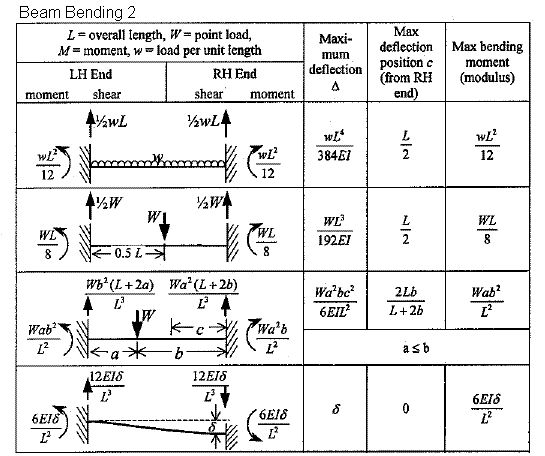
\includegraphics[width=0.6\textwidth]{engineering}
\end{center}%
}{%
\textbf{Calvinball?}
\begin{center}
	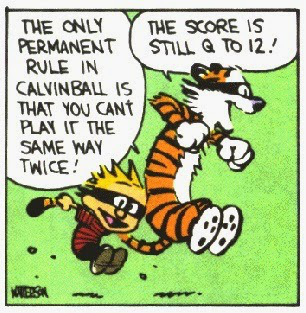
\includegraphics[width=0.6\textwidth]{calvinball}
\end{center}%
}
\end{frame}

\begin{frame}
\frametitle{Engineering} 
For the programmer: simple rule

\begin{quotation}
\textbf{when multiple threads `race' on a variable, tag that variable as atomic}
\end{quotation}

For us:
\begin{enumerate} 
	\item Why is it needed?
	\item What does it do?
	\item (Why) does it work?
\end{enumerate}
\end{frame} 

\begin{frame}
\frametitle{Blame Revisited}
Who is to blame?
\begin{enumerate} 
	\item Programmer/Verifier? \onslide<4->{YES: Missing program annotation}
	\item Compiler? \onslide<3->{YES: Missing fences}
	\item Processor? \onslide<2->{YES: Store buffers (x86,RISCV zTSO,SPARC)}
\end{enumerate}
\end{frame}

\begin{frame}[allowframebreaks]
\frametitle{Enter Storebuffers}
Store Buffer like TODO-List
\begin{center}
\includefig{TODO_empty}
\end{center}
\framebreak
\begin{center}
\includefig{TODO_filling}
\end{center}
\begin{center}
\includefig{TODO_full}
\end{center}
\begin{center}
\includefig{TODO_drain}
\end{center}
\begin{center}
\includefig{buffer_notation}
\end{center}
\end{frame}

\begin{frame}
\frametitle{The Buggy Execution}
Machine Programming Model: (x86,AMD) Store Buffers
\begin{center}\includefig{pres_SB}\end{center}
Too complicated for real programming!
\end{frame} 





\begin{frame}
\frametitle{High Level Programming}
Less Naive Programming Model:

Sequential Consistency (SC) + Software Conditions (SQ)
\begin{center}\includefig{pres_SC_cond}\end{center}
\end{frame}

\begin{frame} 
\frametitle{Software Condition}
Processor level (due to Cohen and Schirmer \cite{cohen_schirmer}):
\begin{quotation}
	\item \textbf{Drain store buffer between racing store and racing load on same thread}
\end{quotation}

\begin{center}
\texttt{
\begin{tabular}{l||l}
\{x\} = i; & \{y\} = i\\ 
\textbf{fence;} & \textbf{fence;}\\
t1 = \{y\}; & t2 = \{x\};
\end{tabular} 
}
\end{center}

Enforced by compiler with knowledge from \texttt{atomic} annotation
\end{frame}



\begin{frame}
\frametitle{Basic Question}
For simple machine (answers in \cite{cohen_schirmer})
\begin{enumerate} 
\item Do the software conditions really always work? YES 
\item Do I need to know about store buffers to program correctly? NO --- obey software conditions in SC 
\end{enumerate}
\end{frame}

\begin{frame}[allowframebreaks]
\frametitle{Main Theorem}
Refinement theorem:

\textbf{If every SC execution of any given program satisfies SQ, then for that program every store buffer machine execution behaves like some SC execution}\\[20pt]

Note:
\begin{enumerate} 
\item ``Behaves like'' means ``every thread sees same values''
\item but steps can be made in a different order
\end{enumerate} 

\framebreak
Example:

\begin{center}
\texttt{
\begin{tabular}{l||l}
\{x\} = 1; & \{y\} = 1; \\
fence; & fence; \\
t1 = \{y\}; & t2 = \{x\}; \\
if (t1 == 0) & if (t2 == 0) \\
\quad z++; & \quad z++; 
\end{tabular}
}
\end{center}

Safe in SC: no race on \texttt{z} since one of \texttt{t1}, \texttt{t2} is not zero

\framebreak



\begin{center}
\begin{tabular}{c c c}
SB & & SC \\ 
\scalebox{.65}{\includefig{pres_thm_example_SB}} & \hspace{2em} & \scalebox{.65}{\includefig{pres_thm_example_SQ}}
\end{tabular}
\end{center}

\framebreak 

\begin{center}
\begin{tabular}{c c c}
SB & & SC \\ 
\scalebox{.65}{\includefig{pres_thm_example_SB_annot}} & \hspace{2em} & \scalebox{.65}{\includefig{pres_thm_example_SQ}}
\end{tabular}
\end{center}

\end{frame}


\begin{frame}
\frametitle{Extended Question}
What are the software conditions for systems code and complex machines?
Is there such a theorem in that setting?

\begin{center}
\begin{tabular}{c|cc}
feature & answered by \\
\hline \\[2pt]
Basic Multicore CPU & \cite{cohen_schirmer} \\
MMUs & \cite{kovalev} \\
Mixed-size accesses with strong HW & \cite{Geng} \\
Mixed-size accesses with real HW & ? \\ 
Misaligned accesses & ? \\
Inter processor/HW interrupts (IPIs) & ? \\
buggy user programs & ? \\
I/O devices with side-effects & ? \\
single cycle fetch\&execute & ? \\
some stores bypass storebuffer & ? \\
\end{tabular}
\end{center}

All of these solved by this paper
\end{frame}


\begin{frame}[allowframebreaks]
\frametitle{Are these features harmless?}

Assume x1,x2 are adjacent bytes in memory
\begin{center}
	\scalebox{.65}{\includefig{defence_two_bytes}}
\end{center}
Use single 16-bit compare-and-swap on \texttt{x1,x2}:
\begin{center}
	\texttt{
		\begin{tabular}{l||l}
			\{x1\} = 1; & (t1,t2) = (\{x1,x2\}).cas(\\
			t3 = x2; & \qquad (0,0) $\rightarrow$ (2,2)); \\
		\end{tabular}
	}
\end{center}
Executions?
\framebreak

Program seems safe in SC+software conditions

\begin{center}
	\begin{tabular}{c c c}
		\scalebox{.65}{\includefig{defence_hetero_race_SQ}} & \hspace{2em} & \scalebox{.65}{\includefig{defence_hetero_race_SQ_alt}}
	\end{tabular}
\end{center}
Observe:
\[ \texttt{t1} = 1  \hspace{1em} \lor \hspace{1em} \texttt{t3}=2 \]
in {\em all} SC executions

\framebreak
In store buffer hardware:
\begin{center}
	\scalebox{.65}{\includefig{defence_hetero_race_SB}}
\end{center}

So in hardware:
\[ \texttt{t1} = 0 \hspace{1em} \land \hspace{1em} \texttt{t3} = 0 \]

Contradicts SC!

\framebreak

Find race in SC?
\begin{enumerate}
	\item Fix definition of race: `` ... and one of them is {\em potentially} modifying''
	\begin{center}
		\scalebox{.65}{\includefig{defence_hetero_race_SQ_new_def}}
	\end{center}
	\framebreak 
	\item With current definition of race? Very tricky (and in the thesis, roughly 80 pages of proof effort):
	Find \textit{delayed} load races between CAS which races with write on same thread
	\begin{center}
		\scalebox{.65}{\includefig{defence_find_hetero_race_SQ}}
	\end{center}
	Prohibit such delayed load races as SC
\end{enumerate} 
\end{frame} 

\begin{frame}
\frametitle{Conclusion}
\begin{itemize} 
	\item Prove program properties in SC
	\item Prove software conditions in SC
	\item Program properties hold on store buffer machines
\end{itemize} 

\begin{quotation} 
	We don't have to teach anybody about store buffers
\end{quotation}
\end{frame} 



\begin{frame} 
\begin{center} 
	Questions?
\end{center}
\end{frame}

\begin{frame} 
\frametitle{C11 --- Races} 
Uses synchronization relation, e.g., annotated write followed by annotated read to same variable 
\begin{center}
	{\includefig{synchronization_relation}}
\end{center}
Unsynchronize accesses to same object $\implies$ undefined behavior!

Correctly finds delayed RMW races

But: 
\begin{quotation}
	``[...] data races, as defined here, and with suitable restrictions on the use of atomics, correspond to data races in a simple interleaved (sequentially consistent) execution.''
\end{quotation}
$\implies$ this is just not correct!
\end{frame}

\begin{frame} 
\frametitle{C11 --- Current Compilers} 
Place memory barrier behind every annotated store

\begin{center}
\begin{tabular}{lcl}
\texttt{\{x\} = 1;} & $\to$ & \texttt{MOV }(into memory); \\
 & & \texttt{MFENCE;}
\end{tabular}
\end{center}

Not needed, very inefficient!

Only needed between annotated store and next annotated load
\end{frame} 

\begin{frame}[allowframebreaks]
\frametitle{Summary of Conditions}
\begin{enumerate} 
\item annotate stores and loads that are racing and ``concurrent'' ({\em no ownership!})
\item flush between annotated store and annotated load on same thread
\item {\em Mixed-Size/Misaligned Acc., Single Cycle F\&E:} forbid delayed RMW races
\begin{center}
\scalebox{.65}{\includefig{defence_find_hetero_race_SQ}}
\end{center}
and annotate delayed store races (like delayed load race, but with 2nd store)
\item {\em IPI:} delivering IPI has to flush store buffers of targets in HW or has unbounded delay
\item {\em Bypassing store buffer:} do not allow annotated store to bypass buffered stores
\item {\em Untrusted (user) code:} flush before entering and after exiting untrusted code
\item {\em I/O device with side effects:} annotate accesses to I/O device with side effects ({\em probably too strong})
\end{enumerate}
\end{frame}

\begin{frame} 
\frametitle{Correctness Proof: overview}

\textbf{If every SC execution of any given program satisfies SQ, then for that program every store buffer machine execution behaves like some SC execution}\\[20pt]


\begin{itemize} 
\item Detect pseudo-races (information sharing) in SC with synchronzation relation
\begin{center}
\scalebox{.3}{\includefig{synchronization}}
\end{center}

\item Look at schedules where a buffered write is never synchronized --- thus never accessed, real machine behaves like SC machine

\item Reorder arbitrary schedule into such a schedule by unrolling in order of global steps 

\end{itemize} 
\end{frame} 




\begin{frame}
\frametitle{Why is this difficult?}
\begin{enumerate}
\item SC and synchronization apply only on SC execution
\item Some features make this very hard, e.g., mixed-size/misaligned accesses
\end{enumerate}
\begin{center}
\begin{tabular}{c c c}
\scalebox{.45}{\includefig{defence_two_bytes_x}} & \hspace{2em} & \scalebox{.6}{\alt<2->
{\alt<3->%
{\includefig{reorder_stuck_cas_race_SB_fail}}%
{\includefig{reorder_stuck_cas_race_SB}}%
}
{\includefig{reorder_stuck_cas_race}}
}
\end{tabular}
\end{center}

\onslide<4-> Show that this never happens using SQ

\end{frame}

\begin{frame}
\frametitle{SQs do not apply!}
In SC: no race!
\begin{center}
\scalebox{.55}{\includefig{reorder_stuck_cas_race_SQ}}
\end{center}

Cohen-Schirmer conditions not strong enough here
\end{frame}

\begin{frame}
\frametitle{SQs do not apply!}
New condition: forbid ``delayed load race''

\begin{center}
\scalebox{.65}{\includefig{defence_find_hetero_race_SQ}}
\end{center}
\onslide<2-> Also does not (immediately) apply:

\begin{center}
\scalebox{.65}{\includefig{reorder_stuck_cas_race_SQ_SC_fail}}
\end{center}
\end{frame}

\begin{frame}
\frametitle{Working hard for SCs}
{\em only to show that such a situation never arises}, sort local steps with \textbf{bubble sort}:
\begin{center}
\scalebox{.55}{\includefig{reorder_stuck_cas_race_SB_sorted}}
\end{center}
\hspace{2em}
\onslide<2->

Then move CAS next to the store...
\begin{center}
\scalebox{.55}{\includefig{reorder_stuck_cas_race_SQ_SC_sorted}}
\end{center}
... and finally obtain contradiction (this slide = 100 pages of proof in thesis)
\end{frame}


\begin{frame}
\frametitle{Detecting Races without Ownership}
Look only at consecutive memory accesses in computations
\begin{center}
\scalebox{.5}{
\begin{tabular}{ccc}
\includefig{pres_SC_race_x} & \hspace{4em} & \includefig{pres_SC_race_y}
\end{tabular}}
\end{center}

Lemma:
If all racing accesses \textbf{found using this method} are annotated, all accesses to same address are synchronized
\begin{center}
\scalebox{.5}{\includefig{synchronization}}
\end{center}
\end{frame} 



\begin{frame} 
\frametitle{Synchronization Proof}
Assume for sake of contradiction accesses to the same address are not synchronized
\begin{center}
\scalebox{.4}{\includefig{no_synchronization}}
\end{center}
Push out all not-synchronized steps...
\begin{center}
\scalebox{.4}{\includefig{no_synchronization_intermediate}}
\end{center}
... until the accesses are consecutive
\begin{center}
\scalebox{.4}{\includefig{no_synchronization_final}}
\end{center}
\end{frame} 



\begin{frame}
\frametitle{Ordered Schedules}
\begin{enumerate} 
\item Call a thread ``dirty'' while it is buffering an annotated write
\item Call an execution ``ordered'' if no ``global step'' is executed while a thread is dirty
\item Lemma: in an ordered execution, an address is not accessed while a thread buffers a write to that address

\begin{center}
\scalebox{.6}{%
\only<1>{\includefig{ordered_no_access_intro}}%
\only<2>{\includefig{ordered_no_access_lock_unlock}}%
\only<3>{\includefig{ordered_no_access_lock_unlock_buf}}%
\only<4->{\includefig{ordered_no_access_lock_unlock_contradiction}}%
}
\end{center}


\onslide<5->{
\item Lemma: in an ordered execution, the processors see the same values as they would in SC

\begin{center}
Ordered execution must look like:
\scalebox{.5}{\includefig{ordered_no_access_lock_unlock_fixed}}

which is equivalent to SC execution:
\scalebox{.5}{\includefig{ordered_no_access_lock_unlock_SQ}}
\end{center}
}
\end{enumerate}
\end{frame} 

\begin{frame}
\frametitle{Arbitrary Schedules}
Idea: unroll schedule in order of ``global steps''

\begin{center}
\scalebox{.55}{\includefig{reorder_no_access_lock_unlock_buf}}
\\[10pt]
\onslide<2->{\scalebox{.55}{\includefig{reorder_no_access_lock_unlock_1}}}
\\[10pt]
\onslide<3->{\scalebox{.55}{\includefig{reorder_no_access_lock_unlock_2}}}
\\[10pt]
\onslide<4->{
\alt<5->{\scalebox{.55}{\includefig{reorder_no_access_lock_unlock_SQ}}}%
{\scalebox{.55}{\includefig{reorder_no_access_lock_unlock_3}}}%
}
\end{center}
\end{frame}

\begin{frame} 
\begin{center} 
Examples
\end{center}
\end{frame}

\begin{frame}[allowframebreaks]
\frametitle{Mixed Size/Misaligned Accesses}
What can go wrong?
Assume x1,x2 are adjacent bytes in memory
\begin{center}
\scalebox{.65}{\includefig{defence_two_bytes}}
\end{center}
Use single 16-bit compare-and-swap on \texttt{x1,x2}:
\begin{center}
\texttt{
\begin{tabular}{l||l}
x1.store(1); & (t1,t2) = (x1,x2).cas(\\
t3 = x2; & \qquad (0,0) $\rightarrow$ (2,2)); \\
\end{tabular}
}
\end{center}
Executions?
\framebreak

Program seems safe in SC+software conditions

(with ownership: switch ownership of \texttt{x2} from \textit{shared} to \textit{read-only}/\textit{owned-shared} on the store)

\begin{center}
\begin{tabular}{c c c}
\scalebox{.65}{\includefig{defence_hetero_race_SQ}} & \hspace{2em} & \scalebox{.65}{\includefig{defence_hetero_race_SQ_alt}}
\end{tabular}
\end{center}
Observe:
\[ \texttt{t1} = 1  \hspace{1em} \lor \hspace{1em} \texttt{t3}=2 \]
in {\em all} SC executions

\framebreak
In store buffer hardware:
\begin{center}
\scalebox{.65}{\includefig{defence_hetero_race_SB}}
\end{center}

So in hardware:
\[ \texttt{t1} = 0 \hspace{1em} \land \hspace{1em} \texttt{t3} = 0 \]

Contradicts SC!

\framebreak

Find race in SC?
\begin{enumerate}
\item Fix definition of race: `` ... and one of them is {\em potentially} modifying''
\begin{center}
\scalebox{.65}{\includefig{defence_hetero_race_SQ_new_def}}
\end{center}
\framebreak 
\item With current definition of race? Very tricky (and in the thesis, roughly 80 pages of proof effort):
Find \textit{delayed} load races between CAS which races with write on same thread
\begin{center}
\scalebox{.65}{\includefig{defence_find_hetero_race_SQ}}
\end{center}
Prohibit such delayed load races as SC
\end{enumerate} 
\end{frame}

\begin{frame}[allowframebreaks]
\frametitle{Code Modification}
Code modification has to be allowed for page swapping
\\[20pt]
Recreates problem from before, but worse:
\begin{center}
\scalebox{.65}{\includefig{pres_SQ_CM}}
\end{center}


\begin{center}
\scalebox{.65}{\includefig{processor_step}}
\end{center}

Beautiful dependent types:
\begin{align*}
F :& \bigcup_i  Val(A_{PR,i}) \times \Sigma_{P,i} \to 2^{ACC_i}
\\
R :& \bigcup_i \Pi core \in Val(A_{PR,i}), x \in \Sigma_{P,i} .
\\ & \qquad Val(F(core,x)) \to D(ACC_{i})
\\
W :& \bigcup_i \Pi core \in Val(A_{PR,i}), x \in \Sigma_{P,i}, fetch \in Val(F(core, x)). 
\\ & \qquad Val(R(core,x,fetch)) \to \bigcup \Set{ PVal(d) | d \in D(ACC_i) } 
\end{align*}
\end{frame}


\begin{frame}[allowframebreaks]
\frametitle{IPI}
IPI with bounded delay:

\begin{center}
\scalebox{0.9}{\includefig{pres_SQ_IPI_example}}
\end{center} 

\begin{center}
\texttt{
\begin{tabular}{l||l}
IC.target = T2; & x = 1; \\
IC.send = 1; & fence; \\
while (IC.send); & \\
t1 = x; & \\
t2 = x; & \\
\end{tabular}
}
\end{center}

In SC (bound = 0) always:
\[ \texttt{t1} \ = \ \texttt{t2} \]
\begin{center}
\begin{tabular}{c c c}
\scalebox{.4}{\includefig{pres_SQ_IPI_x}} & \hspace{2em} & \scalebox{.4}{\includefig{pres_SQ_IPI_no_x}}
\end{tabular}
\end{center}

In SB:
\begin{center}
\scalebox{.4}{\includefig{pres_SB_IPI_x}}
\end{center}
Not obvious how to solve directly in software using SC (needs protocol for handler to communicate IPI reception).

Solutions in thesis:
\begin{enumerate} 
\item Remove IPI bound in SC (IPI can be delayed arbitrarily many instructions)
\item Make \texttt{IPI $\to$ T2} drain buffer of T2, not \texttt{JISR}
\end{enumerate}
\end{frame}

\begin{frame}[allowframebreaks]
\frametitle{Users} 
Flush needed when entering user
\begin{center}
\texttt{
\begin{tabular}{l||l}
x.st(1); & y.st(1); \\
eret; & eret; \\
t1 = y; & t2 = x; \\
\end{tabular}
}
\end{center}

Flush when leaving user? maybe not needed
\framebreak

Programming model SC with user programs: 
\begin{enumerate} 
\item thread does not have store buffer while in trusted code
\item thread has store buffer while in untrusted code
\item memory can be shared arbitrarily with untrusted code, trusted accesses that can race with untrusted accesses must be annotated
\end{enumerate} 

\end{frame} 

\begin{frame}[allowframebreaks]
\frametitle{Device with side effects}
Used, e.g., in Transport-Triggered-Architecture (TTA), and in interrupt controllers

E.g., adder:
\begin{center}
\texttt{
\begin{tabular}{l}
counter = 5; \\
counter = 7;\\
t = counter;
\end{tabular}
}
\end{center}

In SC:
\[ \texttt{t} = 12 \]

In SB forwarding hardware incorrectly predicts
\[ \texttt{t} = 7 \]

\end{frame} 

\bibliography{thesis}

\end{document}